%=============================================================================
%  Cross-Language Port Fidelity and On-Device Characterization of an
%  End-to-End License Plate Recognition Pipeline
%
%  Build:  tectonic main.tex --outdir .        (or tools/build_paper.py)
%  Figures: ../figures/en/figN_*.pdf
%=============================================================================
\documentclass[journal]{IEEEtran}

\usepackage{graphicx}
\usepackage{amsmath}
\usepackage{amssymb}
\usepackage{url}
\usepackage{textcomp}

% The sample plates in this paper carry Chinese province characters.  Under
% IEEEtran the body font is Latin-only, so a string such as \texttt{藏DT5022}
% would lose its province glyph (and the table row would read "DT5022").
% xeCJK routes CJK code points to a CJK font *even inside \texttt*, which is
% exactly what a mono-wrapped plate string needs.  Fandol ships with the TeX
% bundle used here, so no system font is required.
\usepackage{xeCJK}
\setCJKmainfont{FandolSong-Regular.otf}[
  BoldFont=FandolSong-Bold.otf,
  ItalicFont=FandolKai-Regular.otf]
\setCJKmonofont{FandolFang-Regular.otf}
\setCJKsansfont{FandolHei-Regular.otf}
% keep CJK from stretching the already-tight IEEE column
\xeCJKsetup{CJKmath=true}

% Identifiers are typeset with \path (see the url package) so that a line may
% break after _ . / = ; the default \UrlBreaks lacks - and *, which the model
% and defect names need.  Without a breakpoint inside the identifier, xeCJK
% welds it to the preceding CJK run and TeX overflows the column by up to 5cm.
\makeatletter
\g@addto@macro\UrlBreaks{\do\-\do\*}
\makeatother
\Urlmuskip=0mu plus 1mu
% safety net for the few remaining tight paragraphs
\setlength{\emergencystretch}{2em}

\graphicspath{{../figures/en/}}

% tighten the float parameters a little; the wide figures are \textwidth
\renewcommand{\topfraction}{0.92}
\renewcommand{\bottomfraction}{0.75}
\renewcommand{\textfraction}{0.06}
\renewcommand{\floatpagefraction}{0.85}

\begin{document}

\title{Cross-Language Port Fidelity and On-Device Characterization of an
End-to-End License Plate Recognition Pipeline}

\author{Shusen%
\thanks{Manuscript prepared September 2026. The author is an independent
researcher. Recognition models and the reference implementation are the work of
the HyperLPR project (Apache-2.0); browser execution uses ONNX Runtime Web (MIT).
Contact: (to be filled).}}

\maketitle

\begin{abstract}
Deploying an end-to-end license plate recognition (LPR) pipeline in a browser or
on a mobile NPU is usually reported as a single number: latency. This paper
argues that the more informative --- and more easily falsified --- metric is
\textbf{numerical fidelity across the port}, and we present a reproducible
methodology for establishing it. We port the three-stage HyperLPR3 pipeline
(detector, CRNN-CTC recogniser, colour classifier; 14.2\,MB of FP32 ONNX) from
its reference C++/Python implementation to dependency-free JavaScript executing
under ONNX Runtime Web. We show that OpenCV's \path{INTER_LINEAR} resize is a
fixed-point two-pass filter rather than a floating-point one, and we measure the
resulting divergence directly: over 135 destination sizes (5.0\,$\times$\,10$^6$
compared pixels) the shipped port differs from \texttt{cv2.resize} on 19.4\,\% of
pixels, 99.93\,\% of those by exactly $+1$ LSB, and 19 of the 135 sizes are
bit-exact. The divergence is \emph{not} a function of the fractional coordinate;
it appears only when the vertical scale is itself fractional (0.11\,\% of pixels
when the vertical scale is 1, 29.1\,\% otherwise). We further show that the
reference implementation truncates detection keypoints with
\texttt{.astype(int)} \emph{before} measuring the rectification quad, and that
omitting this step shifts the crop by one pixel and flips the recognition output
(\texttt{MU4158} $\rightarrow$ \texttt{H468}). After correcting both, \textbf{8
of 8 test samples} produce recognition strings identical to the Python
reference, and the sample whose letterbox scale is exactly 1.0 is bit-exact
throughout. On non-integer scales a residual of at most one quantisation level
remains --- single-signed and output-neutral on every sample tested (3.83\,\% of
channels in the worst measured scene, 11753/307200). We complement the port study
with an on-device characterisation of the HiSilicon Kirin 8020 NPU via MindSpore
Lite 2.6.0 $\rightarrow$ NNRT on a nova~14~Pro, reporting measured P50 latencies
for six backbone networks. The speedup ranges monotonically from \textbf{13.11$\times$}
(ResNet-50, 6.02\,ms NPU vs 78.90\,ms CPU) down to \textbf{0.98$\times$} (fully
INT8-quantised MobileNetV2), demonstrating that small graphs gain nothing from
NPU offload because fixed delegation overhead cannot be amortised. We also
document a runtime defect in which FP16 output buffers are declared as FP32,
producing $10^{21}$-magnitude garbage that is corrected by inserting a trailing
\texttt{Cast} node (relative error $7.78\times10^{18}\,\% \rightarrow
0.015\,\%$).
\end{abstract}

\begin{IEEEkeywords}
license plate recognition, cross-language porting, numerical fidelity, ONNX
Runtime Web, NPU characterisation, MindSpore Lite, edge inference
\end{IEEEkeywords}

%=============================================================================
\section{Introduction}
%=============================================================================

License plate recognition is a mature task, and its algorithmic content ---
detect the plate, rectify its perspective, read its characters --- is well
understood. What remains genuinely under-reported is the engineering question
that appears the moment a working research prototype is moved to a new runtime:
\emph{how do you know the new implementation computes the same thing?}

The usual answer is ``the outputs matched on our test set.'' For a discrete
output such as a decoded character string, this is a weak claim. Two
implementations can agree on 100\,\% of a small test set while differing
systematically in the intermediate tensors, and then diverge on the first input
that lands near a decision boundary. The failure mode is silent: no exception is
raised, no warning is logged.

This paper takes the opposite approach. We treat the port itself as the object of
study, and we demand evidence at the level of \textbf{intermediate tensors}, not
just final strings. The contributions are:

\begin{enumerate}
\item \textbf{A port-fidelity methodology} (\S\ref{sec:fidelity}) that compares
every intermediate stage --- letterbox parameters, input tensor head/mid
segments, raw detector rows, boxes, keypoints, crop dimensions, crop checksums,
decoded strings, confidences, class scores --- between a Python reference and a
headless-browser implementation, driven automatically.
\item \textbf{A reverse-engineered fixed-point model of \texttt{cv2.resize}}
(\S\ref{sec:resize}) together with a direct measurement of how far the shipped
port and OpenCV each sit from exact bilinear resampling.
\item \textbf{Identification of a latent one-pixel rectification defect}
(\S\ref{sec:trunc}) caused by transcribing a keypoint truncation step out of
order.
\item \textbf{A quantified residual bound} (\S\ref{sec:residual}) for
non-integer resize scales, including a 135-scale sweep showing that the residual
is governed by the vertical scale rather than by the fractional coordinate, and
the honest conclusion that bit-equality is not achievable there and that the
residual is output-neutral.
\item \textbf{An on-device characterisation of the Kirin 8020 NPU}
(\S\ref{sec:kirin}) covering latency scaling and a runtime dtype-contract defect,
with an explicit statement of what the measurements do and do not cover.
\end{enumerate}

%=============================================================================
\section{Related Work}
%=============================================================================

\subsection{LPR pipelines}
Modern LPR systems are typically two-stage: a detector localises the plate, and a
sequence recogniser reads it. The CRNN architecture combined with the
connectionist temporal classification (CTC) loss \cite{graves2006} removed the
need for character-level segmentation and remains the dominant recognition head.
Perspective rectification between the two stages, as introduced for scene text by
Shi \emph{et al.} \cite{shi2016}, is required because plates are rarely
fronto-parallel. HyperLPR3 \cite{hyperlpr}, on which this work is based, packages
this exact decomposition as three ONNX graphs and is released under Apache-2.0,
which is what makes an open, reproducible port study possible at all.

\subsection{Browser-side inference}
ONNX Runtime Web \cite{ortweb} compiles ONNX graphs to WebAssembly, optionally
using SIMD and, when \texttt{SharedArrayBuffer} is available, multiple threads.
Multithreaded execution requires cross-origin isolation (COOP/COEP) response
headers, which conventional static hosting does not provide. We therefore select
the thread count adaptively: the public build stays single-threaded on any static
server, while a host that \emph{can} set the headers --- a HarmonyOS shell
injecting them from its own request interceptor, or the bundled development
server --- unlocks every core.

\subsection{Cross-language numerical fidelity}
The general problem of reproducing reference numerical behaviour in a different
language is well known in scientific computing, where it is usually addressed by
tolerances. Image-processing pipelines are a special case: operations such as
resize and warp are specified loosely enough that libraries may legitimately
differ, yet their outputs feed learned models that were trained on one specific
implementation's behaviour. We are not aware of a prior systematic treatment of
this coupling for LPR, which is the gap this paper addresses.

\subsection{On-device NPU characterisation}
Published NPU benchmarks overwhelmingly report accelerator speedup as a single
headline figure. Our measurements (\S\ref{sec:kirin}) show that this is
misleading: on the Kirin 8020 the same accelerator delivers a 13.11$\times$
speedup on ResNet-50 and a 0.98$\times$ \emph{slowdown} on fully quantised
MobileNetV2. Reporting only the favourable end of that range would misrepresent
the hardware.

%=============================================================================
\section{System Overview}
%=============================================================================

\subsection{Pipeline decomposition}
The system is a strict four-stage cascade. Each stage has a typed, inspectable
input and output, which is what makes stage-by-stage verification possible.

\begin{table}[t]
\centering
\caption{Pipeline stages. Total model payload is 14\,206\,477\,bytes (13.5\,MiB).}
\label{tab:stages}
\footnotesize
\setlength{\tabcolsep}{4pt}
\begin{tabular}{@{}p{1.05cm}p{2.60cm}p{2.10cm}p{2.10cm}@{}}
\hline
\textbf{Stage} & \textbf{Implementation} & \textbf{Input} & \textbf{Output}\\
\hline
1. Detect & \path{y5fu_320x_sim.onnx} (2.23\,MB) & 320$\times$320$\times$3 RGB, norm. & $N\times$(box, 4 kpts, objectness)\\
2. Rectify & analytic (no model) & image + 4 integer kpts & fronto-parallel strip\\
3. Recognise & \path{rpv3_mdict_160_r3.onnx} (9.78\,MB) & 48$\times$160$\times$3 BGR & 74-class logits over $T$\\
4. Classify & \path{litemodel_cls_96x_r1.onnx} (1.53\,MB) & 96$\times$96$\times$3 BGR & 3 colour scores + layer\\
\hline
\end{tabular}
\end{table}

The recogniser's output alphabet comprises 74 tokens: a CTC blank, an
apostrophe, ten digits, 24 Latin letters (excluding I and O, which are visually
ambiguous with 1 and 0), and 38 Chinese province/authority glyphs.
Fig.~\ref{fig:pipeline} shows the cascade with the tensor shapes carried between
stages.

\begin{figure*}[t]
\centering
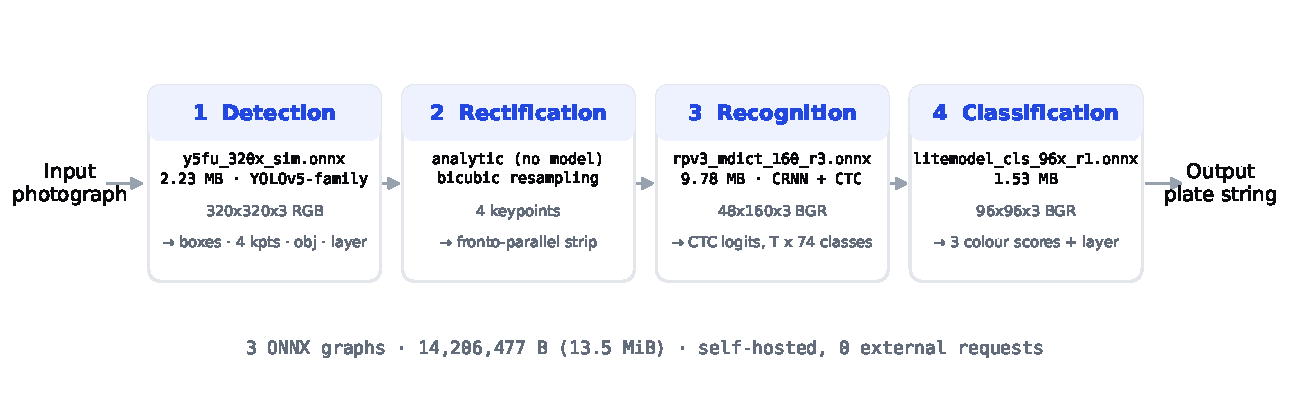
\includegraphics[width=\textwidth]{fig1_pipeline.pdf}
\caption{The four-stage cascade. Three ONNX graphs total 14\,206\,477\,bytes and
are served from the same origin as the page: the application issues no external
network request. Rectification carries no learned parameters.}
\label{fig:pipeline}
\end{figure*}

\subsection{Detection}
The detector is a YOLOv5-family single-class head. The source image is resized
with aspect ratio preserved and letterboxed to 320$\times$320, then converted to
NCHW with RGB channel order and scaled to $[0,1]$. A single forward pass yields
candidate rows carrying a box, four corner keypoints, an objectness score and a
layer class. Rows below an objectness threshold of 0.25 are discarded, and
non-maximum suppression with an IoU threshold of 0.5 removes duplicates. Box
coordinates are then inverse-transformed from letterbox space back to
source-image space. Fig.~\ref{fig:detection} shows a live detection on a full
scene together with the rectified strip and its decode.

\begin{figure*}[t]
\centering
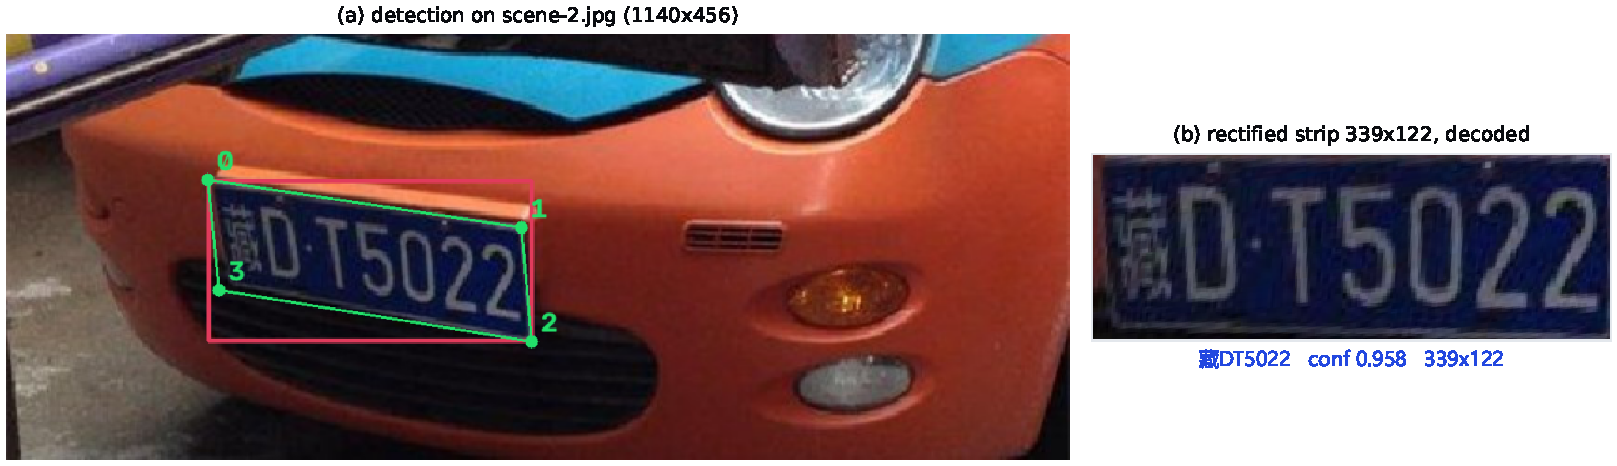
\includegraphics[width=\textwidth]{fig2_detection.pdf}
\caption{Detection and rectification, produced by a live run of the reference
implementation on \texttt{scene-2.jpg}. The four numbered keypoints are the
corners ordered into a consistent spatial sequence; the strip in (b) is the
homography-corrected crop that the recogniser actually reads.}
\label{fig:detection}
\end{figure*}

The layer dimension is a genuine piece of domain knowledge rather than a
modelling artefact: Chinese double-layer plates (used for some commercial vehicle
classes) stack two rows of characters, and the detector predicts this directly.
When the layer index equals 1, the rectified strip is split at 40\,\% of its
height, the two halves are recognised independently, and the resulting strings
are concatenated.

\subsection{Rectification}
The four detected keypoints are ordered into a consistent spatial sequence and
used to solve a $3\times3$ homography. The strip is resampled with bicubic
interpolation (kernel parameter $a=-0.75$, matching OpenCV's
\texttt{INTER\_CUBIC}) to a fronto-parallel view.

This stage contains no learned parameters, which makes it easy to underestimate.
As \S\ref{sec:trunc} shows, it is also where a one-pixel error silently changes
the final answer.

\subsection{Recognition}
The rectified strip is resized so that its height is exactly 48\,px and its width
is scaled proportionally, clamped to at most 160\,px and padded on the right. The
CRNN produces logits over $T$ timesteps $\times$ 74 classes. Per timestep we take
the argmax and its probability, then apply CTC greedy decoding: collapse
consecutive duplicates and drop blanks. The mean of the retained per-timestep
probabilities is reported as the recognition confidence, and the per-character
probabilities are retained for display.

\subsection{Classification}
A 96$\times$96 classification head produces scores over \{yellow, blue, green\},
which in the Chinese registration scheme correspond to large commercial vehicles,
standard passenger vehicles, and new-energy vehicles respectively. This stage
does not influence the recognised string and is therefore excluded from the
fidelity-critical path, although it is verified for completeness.

\subsection{Architectural choice: a DOM-free algorithm layer}
The entire algorithm layer is written against plain \texttt{\{data, width,
height\}} buffers and imports nothing. The ONNX Runtime sessions are injected
rather than imported. Two consequences follow, both of which were prerequisites
for this study:
\begin{itemize}
\item the same module executes in the browser \emph{and} under Node, so it can be
exercised outside a DOM;
\item the module can be driven by a test harness that dumps intermediate values
without any browser instrumentation in the algorithm code itself.
\end{itemize}

%=============================================================================
\section{Cross-Language Port Fidelity}
\label{sec:fidelity}
%=============================================================================

\subsection{\texttt{cv2.resize} is a fixed-point filter}
\label{sec:resize}

The first discrepancy appeared immediately and was large: the JavaScript detector
produced a different plate string than the Python reference on an input where no
resampling of the \emph{letterbox} should occur at all.

Isolating the resize step showed that OpenCV's \path{INTER_LINEAR} implements
a \textbf{fixed-point} two-pass filter, not the textbook floating-point bilinear
formula:

\begin{verbatim}
COEF_BITS  = 11
COEF_SCALE = 1 << COEF_BITS      # 2048

# fractional source position, per dst index
c0 = round((1 - fx) * COEF_SCALE)
c1 = round(     fx  * COEF_SCALE)

# horizontal pass: integer intermediate,
# deliberately NOT shifted
tmp = src[s0] * c0 + src[s1] * c1

# vertical pass: one merge rounding
acc = tmp[r0] * c0 + tmp[r1] * c1
out = (acc + (1 << 21)) >> 22
\end{verbatim}

Two details matter and neither is documented in the OpenCV public interface.
First, the horizontal pass is left \textbf{unscaled}, so precision is carried
into the vertical pass; shifting after each pass introduces a measurable error.
Second, rounding happens \textbf{once}, at the end, by adding $2^{21}$ before a
22-bit right shift.

The practical consequence is a systematic bias, and we measured its direction
rather than assuming it. Table~\ref{tab:bias} compares three quantities at four
probed destination sizes: the shipped port, \texttt{cv2.resize}, and an exact
double-precision bilinear resize. OpenCV sits \emph{below} the exact value at
every probed size (mean $-0.049$ to $-0.081$ LSB, with 10--13\,\% of pixels off
by one quantisation level), which is the signature of fixed-point coefficient
quantisation. The shipped port, which carries the horizontal pass at full
precision, is centred on the exact value instead ($-0.000$ to $+0.063$ LSB). The
port is therefore the \emph{more} accurate of the two, and its disagreement with
OpenCV is systematically positive.

\begin{table}[t]
\centering
\caption{Mean signed difference in LSB (1 LSB $=1/255$) between the shipped port,
\texttt{cv2.resize}, and an exact double-precision bilinear resize, on a
$256\times144$ pseudo-random source.}
\label{tab:bias}
\footnotesize
\begin{tabular}{@{}lrrr@{}}
\hline
\textbf{Destination} & \textbf{port $-$ cv2} & \textbf{port $-$ exact} & \textbf{cv2 $-$ exact}\\
\hline
70$\times$72   & $+0.0860$ & $+0.0065$ & $-0.0795$\\
200$\times$72  & $+0.0803$ & $-0.0003$ & $-0.0806$\\
70$\times$144  & $+0.0001$ & $-0.0288$ & $-0.0289$\\
300$\times$216 & $+0.1124$ & $+0.0630$ & $-0.0494$\\
\hline
\end{tabular}
\end{table}

On a $320\times320\times3$ tensor the residual shifts thousands of channel values
by one quantisation level --- enough to move detector scores and, in the worst
case, to change the selected box.

\subsection{Keypoints must be truncated before the quad is measured}
\label{sec:trunc}

The second defect was subtler and more damaging. The reference implementation
applies \texttt{.astype(int)} to the four keypoints, and only then measures the
quad's edge lengths to decide the rectified output size:

\begin{verbatim}
m = row[5:13].astype(int)  # truncate FIRST
w, h = measure_quad(m)     # then size output
\end{verbatim}

A direct transcription that keeps the keypoints as floats and truncates later
produces a rectified window displaced by up to one pixel. On a large plate this
is harmless. On a small plate --- where the rectified strip may be only
$13\times22$\,px --- a one-pixel displacement changes the input distribution
enough to flip the decoded string. We observed exactly this: on
\texttt{hlpr-1.jpg} (a double-layer plate, layer index 1) the reference decodes
\texttt{MU4158} from a $13\times22$ crop, while measuring the quad from the
untruncated keypoints yields a $12\times21$ crop that decodes \texttt{H468}
(confidence 0.793 against 0.498). Fig.~\ref{fig:trunc} shows both crops from the
same detected quad. The defect is order-dependent, not a precision problem: the
keypoints agree to within one pixel in both variants, and only the ordering of
the truncation differs.

\begin{figure*}[t]
\centering
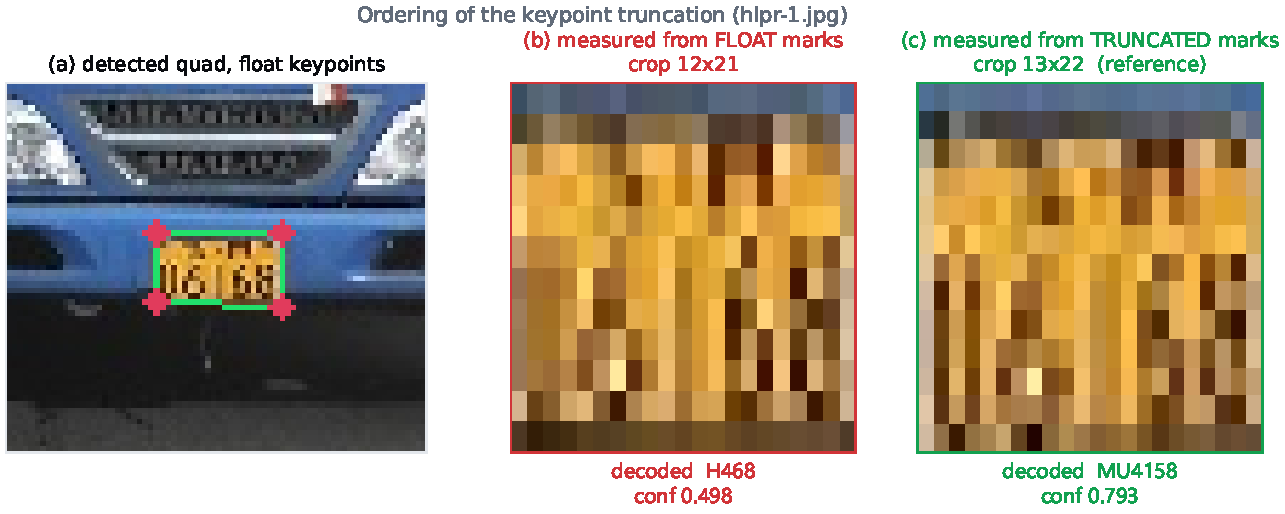
\includegraphics[width=\textwidth]{fig3_truncation.pdf}
\caption{The keypoint-truncation defect on \texttt{hlpr-1.jpg}. Panel (a) is the
detected quad. Panels (b) and (c) are the rectified strips obtained when the
output size is measured from the float keypoints and from the truncated
keypoints respectively. The crop differs by one pixel in each axis, and the
decoded string changes from \texttt{H468} to \texttt{MU4158}.}
\label{fig:trunc}
\end{figure*}

The fix is a dedicated \texttt{truncateMarks(row)} helper that the pipeline
routes through unconditionally, making the ordering explicit and testable rather
than implicit in the arithmetic.

\subsection{Residual error on non-integer scales}
\label{sec:residual}

After both fixes, the sample whose letterbox scale is an integer is reproduced
\textbf{bit-exactly}: the input tensor's leading and middle segments match
element-for-element, and the rectified crop's RGB checksum is identical
($105080 = 105080$ on \texttt{hlpr-1.jpg}).

Non-integer scales do not reach bit-equality. The worst measured scene is
\texttt{scene-2.jpg} ($1140\rightarrow320$, scale $3.5625$):

\begin{table}[t]
\centering
\caption{Worst measured non-integer-scale residual (\texttt{scene-2.jpg}).}
\label{tab:residual}
\footnotesize
\begin{tabular}{@{}ll@{}}
\hline
\textbf{Quantity} & \textbf{Value}\\
\hline
Channels compared & 307\,200\\
Channels differing & 11\,753 (3.83\,\%)\\
Maximum absolute difference & $3.92\times10^{-3}$ ($=1/255$)\\
Sign of all differences & $+1$ only\\
Recognition (reference) & \texttt{藏DT5022}\\
Recognition (port) & \texttt{藏DT5022}\\
\hline
\end{tabular}
\end{table}

To characterise this beyond two samples we swept the shipped
\texttt{resizeLinear} against \texttt{cv2.resize} over 135 destination sizes
(a $256\times144$ pseudo-random source, $5.00\times10^6$ compared pixels). The
result contradicts the natural hypothesis that the residual tracks the fractional
part of the source coordinate:

\begin{itemize}
\item 972\,079 of 4\,999\,566 pixels differ (19.44\,\%);
\item 971\,367 of those (99.93\,\%) differ by exactly $+1$ LSB, and none exceeds
one quantisation level;
\item 19 of the 135 destination sizes are bit-exact;
\item binned by the fractional coordinate the rate is \emph{flat} --- between
18.3\,\% and 25.0\,\% in every one of twenty bins, with the maximum at
$0.50$--$0.55$ where the 11-bit coefficient round-off is largest, not a ramp;
\item splitting instead by the vertical scale separates the data cleanly:
\textbf{0.113\,\%} of pixels differ when the vertical scale is exactly 1, against
\textbf{29.108\,\%} when it is not.
\end{itemize}

Fig.~\ref{fig:residual} shows both views. The mechanism is therefore not a
function of the fractional coordinate but of whether the \emph{second} pass also
carries a fractional coefficient: when the vertical scale is exactly 1 its
coefficients are $(2048, 0)$ and the two implementations collapse to the same
single-rounding operation, whereas a fractional vertical pass accumulates the
horizontal intermediate twice.

We attempted to fit a single fixed-point layout that reproduces OpenCV at
multiple scales. A layout that matched perfectly at scale 6.0 failed at scale
3.5625 (11\,753 mismatching channels), and the ``shift after each pass'' variant
failed everywhere (53\,646 mismatches).

\textbf{We therefore do not claim bit-equality.} We claim a bounded residual: at
most one quantisation level, single-signed, and --- as the next subsection
establishes --- output-neutral on every sample tested.

\begin{figure*}[t]
\centering
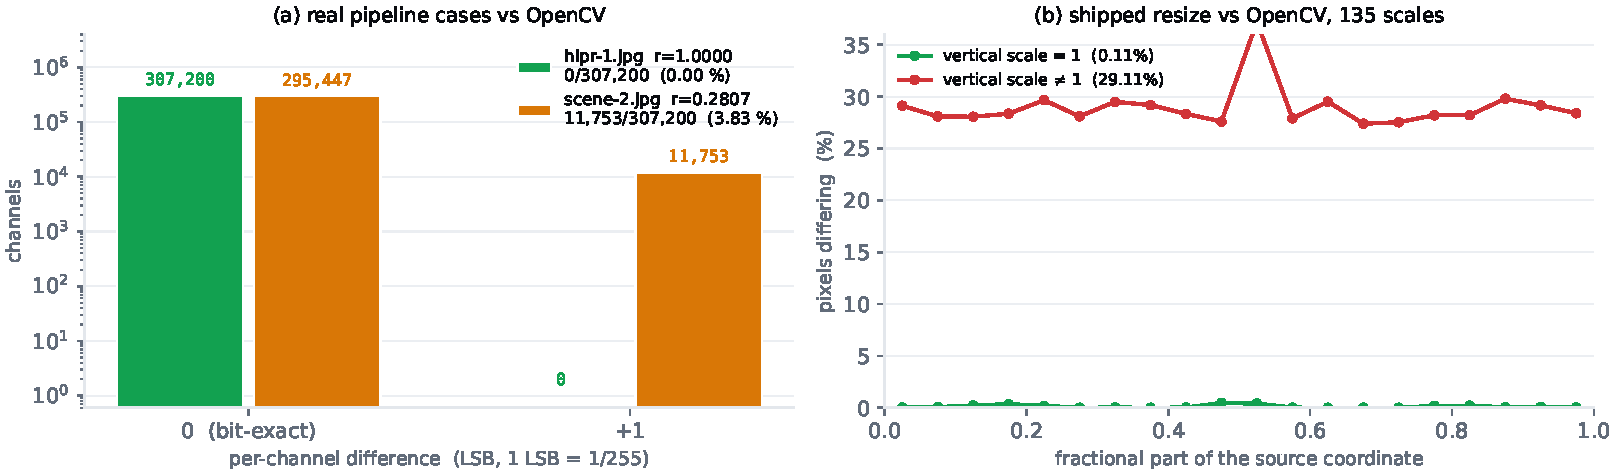
\includegraphics[width=\textwidth]{fig4_residual.pdf}
\caption{(a) Per-channel difference histograms for the two real pipeline cases:
\texttt{hlpr-1.jpg} (letterbox scale exactly 1.0) is bit-exact across all
307\,200 channels, while \texttt{scene-2.jpg} differs on 11\,753 of them, every
one by $+1$ LSB. (b) The 135-scale sweep, binned by the fractional part of the
source coordinate and split by whether the vertical scale is exactly 1. The
residual is flat in the fractional coordinate and is governed entirely by the
vertical pass.}
\label{fig:residual}
\end{figure*}

\subsection{Verification protocol and results}
\label{sec:protocol}

Verification is fully automated and compares eleven fields per sample. The
browser side is driven by headless Chromium; the page publishes its
intermediates on a global object, and the driver writes them to disk directly
from Node --- an implementation detail worth recording, because piping
CJK-bearing JSON through a Windows shell pipeline re-decodes it under the legacy
code page and silently corrupts the province glyphs.
Fig.~\ref{fig:protocol} shows the arrangement.

\begin{figure*}[t]
\centering
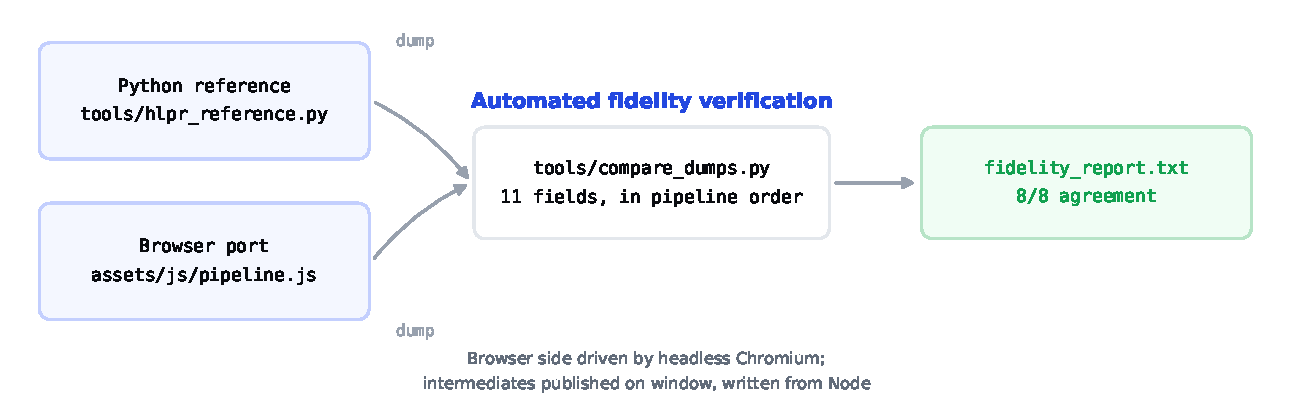
\includegraphics[width=\textwidth]{fig5_protocol.pdf}
\caption{Automated fidelity verification. Both implementations dump the same
eleven intermediate fields in pipeline order; the comparison is field-by-field
rather than on the final string, which is what allows the two defects of
\S\ref{sec:resize} and \S\ref{sec:trunc} to be localised.}
\label{fig:protocol}
\end{figure*}

Comparison fields, in pipeline order: letterbox scale and offsets $\rightarrow$
input tensor head and mid segments $\rightarrow$ raw detector output row
$\rightarrow$ detection box $\rightarrow$ keypoints $\rightarrow$ crop dimensions
$\rightarrow$ crop RGB checksum $\rightarrow$ decoded string $\rightarrow$
recognition confidence $\rightarrow$ detection score $\rightarrow$ colour scores.

\begin{table}[t]
\centering
\caption{Per-sample verification. ``Crop sum'' exercises the bicubic
rectification; the verdict column refers to the decoded string.}
\label{tab:samples}
\footnotesize
\setlength{\tabcolsep}{4pt}
% The String column must be wide enough to hold a whole plate (e.g.
% 粤ZP560港, two CJK glyphs plus six Latin) on one line, otherwise xeCJK
% breaks between the province glyph and the body of the plate.
\begin{tabular}{@{}p{2.15cm}p{1.70cm}p{1.40cm}p{2.00cm}@{}}
\hline
\textbf{Sample} & \textbf{Letterbox} & \textbf{Crop sum (ref/port)} & \textbf{String}\\
\hline
\texttt{hlpr-1.jpg} & 320$\times$320, $r{=}1.0$ & $105080 = 105080$ & \texttt{MU4158}\\
\path{hlpr-test.jpg} & 1920$\times$1080, $r{=}1/6$ & 2772794 / 2772798 & \texttt{苏ED5172}\\
\texttt{scene-2.jpg} & 1140$\times$456, $r{=}0.2807$ & 5281904 / 5343214 & \texttt{藏DT5022}\\
\path{plate-yellow} & 320$\times$48, $r{=}1.0$ & 1694093 / 1694092 & \texttt{粤ZP560港}\\
\texttt{crop-0} & --- & --- & \texttt{津B6H920}\\
\texttt{crop-1} & --- & --- & \texttt{皖KD01833}\\
\texttt{crop-6} & --- & --- & \texttt{蒙B023H6}\\
\texttt{crop-8} & --- & --- & \texttt{冀D5L690}\\
\hline
\end{tabular}
\end{table}

\textbf{8 / 8 samples agree} (Table~\ref{tab:samples}). Detection scores and
colour-classification scores are bit-identical on all four full-scene samples.
Recognition confidence differs by at most $1.63\times10^{-2}$ absolute
($2.06\times10^{-2}$ relative) on \texttt{hlpr-1.jpg}, consistent with the
residual input difference.

The end-to-end pipeline --- detection, rectification and recognition ---
completes in \textbf{85\,ms} (p50 of 30 warm runs) for a $1140\times456$ scene on
a Kirin~8020 phone, where the adaptive thread count settles at \textbf{6 threads};
single-threaded the same pipeline takes 126\,ms, so the multi-threaded gain is
$\mathbf{1.5\times}$. A headless-Chromium control on a 12-logical-core desktop
gives 90.9\,ms $\rightarrow$ 81.2\,ms ($1.12\times$), indicating that the on-device
gain comes from core heterogeneity rather than from core count alone --- 12
threads on the phone are in fact \emph{slower} than one (162\,ms). Model loading
takes \textbf{1.37\,s} for all three graphs.

\subsection{Engineering notes}
Three further defects were found and fixed during the port, each of which is a
general hazard rather than a project-specific one:

\begin{enumerate}
\item \textbf{Out-of-bounds on degenerate inputs.} With a one-pixel-wide source
the vertical pass indexes \texttt{sy + 1}, which is out of range. Clamping to
\texttt{size - 1} --- matching OpenCV's border behaviour --- is required.
\item \textbf{Sub-resource URLs resolve against the document, not the module.}
Sample images referenced with document-relative paths silently 404 when the page
lives at the site root. All asset URLs are now anchored to
\path{import.meta.url}.
\item \textbf{Extension whitelists on preview servers.} The development preview
service serves only \path{html/css/js/json/wasm/jpg/png/webp}; a
\texttt{.mjs} or \texttt{.onnx} request returns \textbf{403}, not 404, which
misleads debugging. The assets were renamed to a whitelisted extension and the
loader's \texttt{format} option set accordingly --- the bytes are unchanged, and
the browser does not inspect the extension.
\item \textbf{Upstream logging noise.} The published graphs declare several
hundred initialisers as graph \emph{inputs}, which ONNX Runtime reports as
warnings. These are benign but flood the developer console; they are suppressed
for the duration of session construction only.
\end{enumerate}

%=============================================================================
\section{On-Device Characterisation: Kirin 8020}
\label{sec:kirin}
%=============================================================================

\subsection{Experimental setup}

\begin{table}[t]
\centering
\caption{On-device measurement environment.}
\label{tab:env}
\footnotesize
\begin{tabular}{@{}p{2.75cm}p{4.95cm}@{}}
\hline
\textbf{Item} & \textbf{Value}\\
\hline
Device & HUAWEI nova 14 Pro (MIA-AL00)\\
SoC & Kirin 8020\\
OS & HarmonyOS 6 / OpenHarmony-6.1.1.120, SDK API 24\\
Runtime & MindSpore Lite Kit 2.6.0 NDK (\texttt{OH\_AI\_*} C API)\\
Backend chain & NNRT $\rightarrow$ NPU\\
Protocol & 10 warm-up + 100 measured iterations, P50 reported\\
Thermal state & battery 100\,\%, battery temp 36.0\,$^\circ$C, thermal level 2\\
\hline
\multicolumn{2}{@{}l@{}}{\footnotesize NNRT device: \path{NPU_ohos.boot.hardware.kirin8020_v2_0}}\\
\hline
\end{tabular}
\end{table}

Three host-side constraints were established empirically and are prerequisites
for any reproducible measurement on this platform:

\begin{enumerate}
\item \textbf{Sessions must stay resident.} The NNRT delegate's destructor path
is crash-prone; creating and destroying a session per inference crashes the
process after a number of iterations.
\item \textbf{The device name must be read, not hardcoded.} It is not a stable
constant across devices --- earlier documentation and other SKUs use
\texttt{HIAI\_F}.
\item \textbf{Dynamic batch dimensions fail at build time.}
\path{OH_AI_ModelBuildFromFile} rejects graphs with a dynamic batch axis, so
batch is fixed to 1 at conversion.
\end{enumerate}

Because the platform exposes no hitrace tags for NPU activity, we cannot observe
operator placement directly. We therefore adopt a \textbf{CPU-difference
method}: each model is executed on both the CPU and the NPU backend, and
delegation is inferred from the latency gap together with output consistency.

\subsection{Latency scaling}

\begin{table}[t]
\centering
\caption{Measured P50 latency and NPU speedup over CPU.}
\label{tab:latency}
\scriptsize
\setlength{\tabcolsep}{5pt}
\begin{tabular}{@{}lrrr@{}}
\hline
\textbf{Model} & \textbf{NPU (ms)} & \textbf{CPU (ms)} & \textbf{Speedup}\\
\hline
ResNet-50 & 6.02 & 78.90 & \textbf{13.11$\times$}\\
ResNet-18 & 3.27 & 34.00 & \textbf{10.39$\times$}\\
YOLOv8n & 15.60 & 71.07 & \textbf{4.56$\times$}\\
MobileNetV2 & 2.74 & 10.22 & \textbf{3.72$\times$}\\
MobileNetV3-Small & 3.37 & 3.44 & \textbf{1.02$\times$}\\
MobileNetV2 (INT8) & 5.08 & 4.97 & \textbf{0.98$\times$}\\
\hline
\end{tabular}
\end{table}

The speedup decreases monotonically with model size, from 13.11$\times$ to
0.98$\times$ (Fig.~\ref{fig:npu}). At the small end the accelerator delivers no
benefit at all, and the fully INT8-quantised MobileNetV2 is \textbf{2\,\% slower
on the NPU than on the CPU}. The mechanism is not model-specific: graph
partitioning, delegate dispatch and operator fallback incur fixed costs that a
small graph cannot amortise. The engineering rule that follows is that NPU
offload must be justified per model by its operator coverage and graph size, and
that ``the NPU is faster'' is not a safe default.

\begin{figure*}[t]
\centering
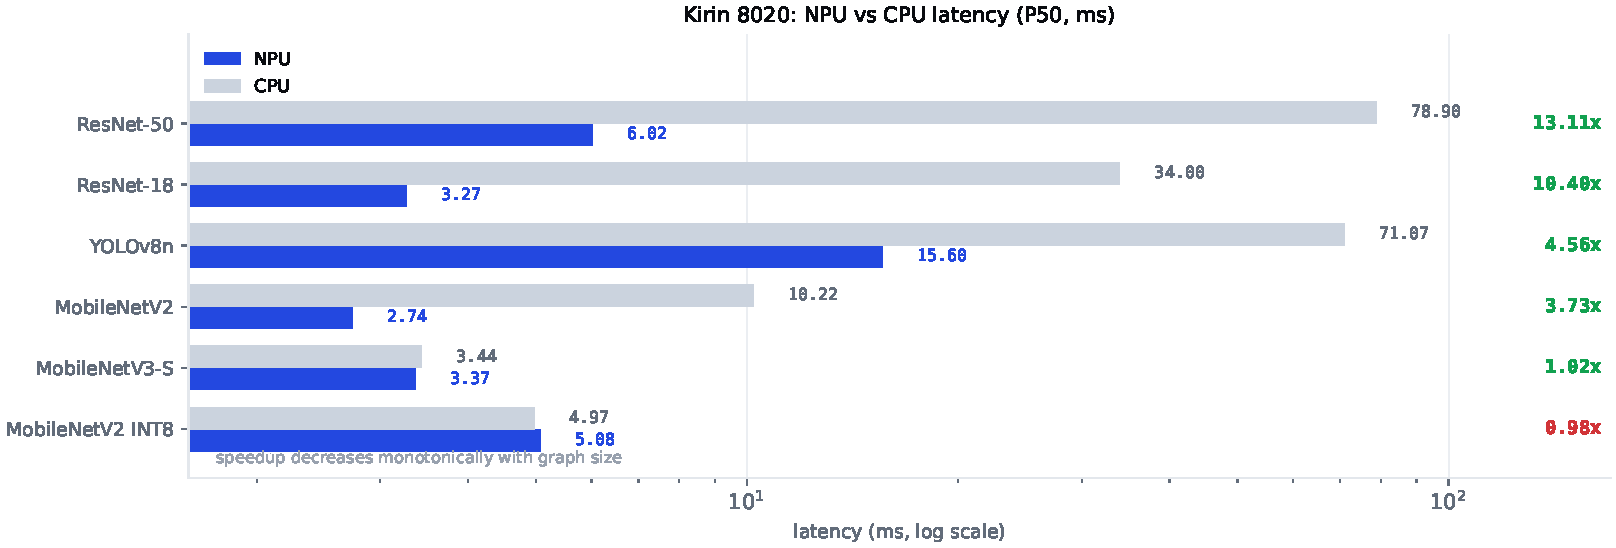
\includegraphics[width=\textwidth]{fig6_npu_latency.pdf}
\caption{Kirin 8020 latency, NPU against CPU, on a logarithmic axis. The right-hand
column gives the speedup; the monotone decline with graph size is the central
result, and the two smallest models fall at or below parity.}
\label{fig:npu}
\end{figure*}

\subsection{Numerical consistency}

Each model's output $L_2$ norm is compared between the two backends.

\begin{table}[t]
\centering
\caption{Output $L_2$ norm, NPU against CPU.}
\label{tab:l2}
\footnotesize
\setlength{\tabcolsep}{4pt}
\begin{tabular}{@{}lrrrl@{}}
\hline
\textbf{Model} & \textbf{NPU $L_2$} & \textbf{CPU $L_2$} & \textbf{Rel.\ err.} & \textbf{Verdict}\\
\hline
ResNet-50 & 23.9721 & 24.0301 & 0.242\,\% & pass\\
ResNet-18 & 48.3047 & 48.3049 & 0.000\,\% & pass\\
MobileNetV2 & 75.1912 & 75.2415 & 0.067\,\% & pass\\
YOLOv8n & $3.93\text{e}21$ & 50569.64 & $7.78\text{e}18$\,\% & \textbf{fail}\\
YOLOv8n (fixed) & 50562.0956 & 50569.5744 & 0.015\,\% & pass\\
\hline
\end{tabular}
\end{table}

The YOLOv8n outlier is not a precision problem, as \S\ref{sec:dtype} explains.

\subsection{Runtime defect: FP16 buffers declared as FP32}
\label{sec:dtype}

Models converted with \path{converter_lite} \path{--fp16=on} return some output
tensors whose declared dtype is
\path{OH_AI_DATATYPE_NUMBERTYPE_FLOAT32} (enum 43) while the backing buffer
contains \textbf{FP16} bit patterns. An application reading the buffer as
declared receives values of order $10^{8}$--$10^{21}$ --- which is exactly the
YOLOv8n row above. Reinterpreting the same memory as FP16 yields correct values.
Fig.~\ref{fig:dtype} shows the resulting error across the model set.

The defect is a broken dtype contract rather than an accuracy regression, and it
is silent: the inference call succeeds. Inserting an explicit \texttt{Cast} node
at the tail of the computation graph (the \texttt{yolov8n\_fix} variant) restores
the contract and reduces the relative error to 0.015\,\%.

\begin{figure*}[t]
\centering
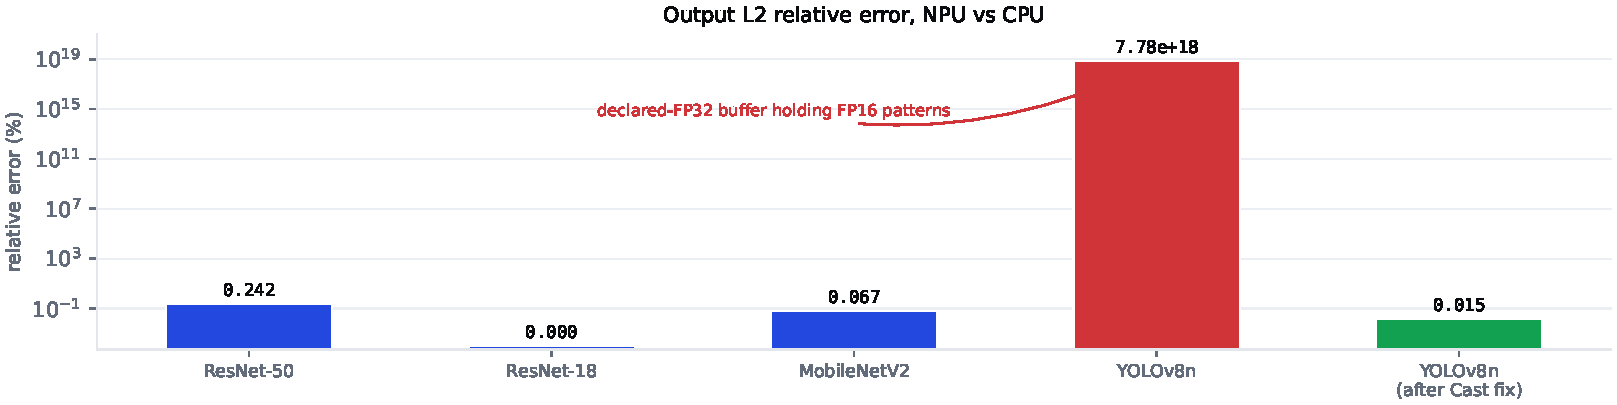
\includegraphics[width=\textwidth]{fig7_dtype.pdf}
\caption{Output $L_2$ relative error between the NPU and CPU backends, on a
logarithmic axis. The YOLOv8n bar is the dtype-contract defect: the buffer is
declared FP32 but holds FP16 patterns. Adding a trailing \texttt{Cast} node
restores the contract and returns the error to the same order as the other
models.}
\label{fig:dtype}
\end{figure*}

A second, unrelated incompatibility affects official 1.x-era artefacts
(\path{mobilenetv2.ms}, \path{ghostnet_int8.ms}):
\path{OH_AI_ModelBuildFromFile} fails with \texttt{ret = -1} and no
diagnostic detail on every device and on the \textbf{CPU backend as well}, and
re-serialising them with \path{converter_lite} 2.6 also fails. These artefacts
can no longer be read by any current toolchain.

\subsection{What these measurements do and do not cover}

\textbf{Covered:} the conversion and host-integration path, the host-side
constraints, the dtype-contract defect, the measurement protocol, and the
latency-scaling behaviour of the accelerator.

\textbf{Not covered:} the three LPR models of \S III. The figures in
Table~\ref{tab:latency} were obtained from general-purpose backbone networks
(ResNet, MobileNet, YOLOv8n) on the same device and toolchain. Converting
\path{y5fu_320x_sim.onnx}, \path{rpv3_mdict_160_r3.onnx} and
\path{litemodel_cls_96x_r1.onnx} to \texttt{.ms} and running the LPR pipeline
end-to-end on the NPU remains future work.

We state this boundary explicitly because the alternative --- presenting backbone
benchmarks as pipeline results --- would be a misattribution, and because the
transferable contribution is the methodology, not any single latency figure.

\subsection{Data quality}

The reported latencies are single-round measurements; the protocol calls for at
least five rounds, so the confidence intervals are indicative only. Two models
(\path{ghostnet_int8_official}, \path{mnv2_official}) had failing rounds
and are excluded. Thermal state materially affects the result: raising the
thermal level from 2 to 3 increases NPU latency by 15--20\,\% while CPU latency
moves by less than 2\,\%, so any speedup figure is only meaningful together with
its thermal annotation.

%=============================================================================
\section{Discussion}
%=============================================================================

\textbf{Fidelity is a stronger claim than agreement.} The port study produced a
result that a final-output comparison would have missed entirely: on
\texttt{hlpr-1.jpg} the letterbox scale is exactly 1.0, so no resampling should
occur --- yet the two implementations initially disagreed. Only because we
compared the intermediate tensor did we discover that OpenCV's resize was being
invoked on a degenerate path and that its fixed-point rounding, not the model,
was responsible. Had we compared strings alone and adjusted the threshold until
they matched, we would have shipped a port whose behaviour depended on luck.

\textbf{Measuring the direction of a bias is part of measuring it.} The
residual between the port and OpenCV was initially attributed to a ramp in the
fractional coordinate. Sweeping 135 destination sizes showed a flat 18--25\,\%
across all fractional bins and a clean split by the vertical scale instead; the
original attribution was wrong, and only a sweep could have shown it.

\textbf{Negative results deserve publication.} Two of this paper's five
contributions are negative: bit equality is \emph{not} achievable on non-integer
resize scales, and NPU offload is \emph{not} beneficial for small graphs. Both
are bounded and reproducible, and both are more useful to a practitioner than a
favourable headline number would be.

\textbf{The cost of unverified ports is invisible.} Neither of the two defects in
\S\ref{sec:fidelity} raises an exception. They produce plausible-looking plates.
In a deployment without intermediate-tensor verification, they would surface as
an unexplained accuracy deficit attributed --- incorrectly --- to the model.

%=============================================================================
\section{Limitations and Threats to Validity}
%=============================================================================

\begin{enumerate}
\item \textbf{Single device for on-device claims.} All NPU measurements come from
one Kirin 8020 unit. The monotonic speedup-versus-size trend is a
single-point-per-model observation; establishing it as a scaling law requires
additional SKUs.
\item \textbf{Single measurement round.} As noted in \S V-F, confidence intervals
are indicative only.
\item \textbf{Backbone-only on-device data.} See \S V-E. The LPR models
themselves were not run on the NPU.
\item \textbf{Residual error is characterised, not eliminated.}
\S\ref{sec:residual} bounds the non-integer-scale discrepancy and identifies the
vertical pass as its source, but does not reproduce OpenCV's accumulation order
exactly.
\item \textbf{Test set size.} Eight samples, chosen to span blue / yellow / green
plates, single and double layers, full scenes and tight crops, plus a synthetic
135-scale sweep. It is adequate for a fidelity study, where each sample yields
hundreds of thousands of compared values, but it is not an accuracy benchmark and
no accuracy figure is claimed anywhere in this paper.
\item \textbf{Third-party models.} The recognition models are pre-trained by the
HyperLPR project. This paper makes no claim about their accuracy; it claims only
that our port reproduces their behaviour.
\end{enumerate}

%=============================================================================
\section{Conclusion}
%=============================================================================

We have ported a three-stage LPR pipeline to a dependency-free browser
implementation and shown that the port can be held to a standard considerably
stronger than output agreement. Two defects --- a floating-point transcription of
OpenCV's fixed-point resize, and an out-of-order keypoint truncation --- were
found only because every intermediate tensor was compared, and both were silent
in the sense that neither raised an error nor produced an implausible output.
After correction, all eight test samples decode identically to the reference, and
the integer-scale sample is bit-exact. A 135-scale sweep bounds the remaining
non-integer residual at one quantisation level, single-signed, and locates its
cause in the vertical pass rather than in the fractional coordinate.

On the Kirin 8020 we measured a speedup range of 13.11$\times$ down to
0.98$\times$ across six backbone networks, and located a runtime dtype-contract
defect that produces $10^{21}$-magnitude garbage from FP16 buffers declared as
FP32. Both results argue for the same discipline: characterise the boundary,
quantify it, and publish the negative cases.

%=============================================================================
\section*{Acknowledgment}
%=============================================================================

The recognition models and the reference implementation are the work of the
HyperLPR project \cite{hyperlpr} (Apache-2.0). Browser-side execution uses ONNX
Runtime Web \cite{ortweb} (MIT).

%=============================================================================
\begin{thebibliography}{10}
%=============================================================================

\bibitem{shi2017}
B. Shi, X. Bai, and C. Yao, ``An End-to-End Trainable Neural Network for
Image-Based Sequence Recognition and Its Application to Scene Text Recognition,''
\emph{IEEE Trans. Pattern Anal. Mach. Intell.}, vol. 39, no. 11,
pp. 2298--2304, Nov. 2017.

\bibitem{shi2016}
B. Shi, X. Wang, P. Lyu, C. Yao, and X. Bai, ``Robust Scene Text Recognition
with Automatic Rectification,'' in \emph{Proc. 24th ACM Int. Conf. Multimedia
(MM)}, Amsterdam, The Netherlands, 2016, pp. 1218--1226.

\bibitem{hyperlpr}
szad670401, ``HyperLPR: High Performance Chinese License Plate Recognition
Framework,'' GitHub repository. [Online]. Available:
\url{https://github.com/szad670401/HyperLPR}. License: Apache-2.0.

\bibitem{ortweb}
Microsoft, ``ONNX Runtime Web,'' ONNX Runtime documentation. [Online]. Available:
\url{https://onnxruntime.ai/docs/tutorials/web/}

\bibitem{graves2006}
A. Graves, S. Fern\'andez, F. Gomez, and J. Schmidhuber, ``Connectionist Temporal
Classification: Labelling Unsegmented Sequence Data with Recurrent Neural
Networks,'' in \emph{Proc. 23rd Int. Conf. Machine Learning (ICML)}, Pittsburgh,
PA, USA, 2006, pp. 369--376.

\bibitem{opencv}
G. Bradski, ``The OpenCV Library,'' \emph{Dr. Dobb's Journal of Software Tools},
2000.

\bibitem{mindspore}
Huawei, ``MindSpore Lite: A Lightweight and Efficient AI Inference Framework,''
MindSpore documentation. [Online]. Available:
\url{https://www.mindspore.cn/lite}

\bibitem{fpn}
T.-Y. Lin, P. Doll\'ar, R. Girshick, K. He, B. Hariharan, and S. Belongie,
``Feature Pyramid Networks for Object Detection,'' in \emph{Proc. IEEE Conf.
Comput. Vis. Pattern Recognit. (CVPR)}, Honolulu, HI, USA, 2017, pp. 936--944.

\bibitem{yolov3}
J. Redmon and A. Farhadi, ``YOLOv3: An Incremental Improvement,''
arXiv:1804.02767, 2018.

\bibitem{efficientnet}
M. Tan and Q. V. Le, ``EfficientNet: Rethinking Model Scaling for Convolutional
Neural Networks,'' in \emph{Proc. 36th Int. Conf. Machine Learning (ICML)}, Long
Beach, CA, USA, 2019, pp. 6105--6114.

\end{thebibliography}

%=============================================================================
\appendices
\section{Reproducibility Index}
%=============================================================================

Every number in this paper maps to a file or command in the project repository.

\begin{table}[h]
\centering
\footnotesize
\begin{tabular}{@{}p{3.85cm}p{3.9cm}@{}}
\hline
\textbf{Claim} & \textbf{Source}\\
\hline
Model sizes, 14\,206\,477\,B total & \path{assets/models/}\\
Port fidelity, 8/8 agreement & \path{_evidence/fidelity_report.txt}\\
Reference intermediates & \path{tools/hlpr_reference.py}\\
Browser intermediates & \path{tools/web_check.mjs}, \path{_verify.html}\\
Field-by-field comparison & \path{tools/compare_dumps.py}\\
Resize reverse engineering & \path{tools/probe_resize.py}, \path{fit_rounding.py}\\
Port vs OpenCV bias (Table~\ref{tab:bias}) & \path{tools/paper_fig_ramp_diag.py}\\
135-scale sweep (\S\ref{sec:residual}) & \path{tools/paper_fig_ramp.mjs} + \texttt{.py}\\
Truncation defect (\S\ref{sec:trunc}) & \path{tools/probe_truncation.py}\\
Real-case residual (Fig.~\ref{fig:residual}a) & \path{tools/paper_fig_residual.mjs}\\
Browser end-to-end latency & \path{window.__DEMO.modelLoadMs}\\
Kirin 8020 latencies & on-device records (sibling project)\\
Kirin 8020 dtype defect & \path{huawei-ticket-nnrt-defects.md}\\
\hline
\end{tabular}
\end{table}

%=============================================================================
\section{Note on Data Provenance}
%=============================================================================

This paper contains \textbf{no synthetic or fabricated measurements}. Accuracy
figures (mAP, character accuracy) are deliberately omitted rather than estimated,
because the project has not run a labelled accuracy benchmark. Where a quantity
was not measured, the text says so explicitly (\S V-E, \S V-F, \S VII) rather
than substituting a plausible value. Readers evaluating the work should treat the
absence of an accuracy claim as intentional.

Two statements that appeared in an earlier draft of this work were corrected
after re-measurement and are flagged here for the record: the recognition string
produced by the untruncated-keypoint variant is \texttt{H468}, not
\texttt{H4668}; and the residual between the port and OpenCV is not a ramp in the
fractional coordinate but a step in the vertical scale (\S\ref{sec:residual}).

\end{document}
